\section{Part 2: ANDi Tool and Automotive Ethernet }
\label{sec:mediagateway}

This section details the establishment of a communication path.

\subsection{Simple Connection Setup}
% Describe the physical and logical setup for a simple connection. 
A simple setup typically means connecting two or more devices through the gateway, which acts as an intermediary for data transmission. For that devices are physically linked to the MediaGateway’s network ports using twisted pair cables and MediaConverters. The MediaGateway acts as a Layer 2 switch in this setup, forwarding Ethernet frames between connected devices without complex routing. Each device connects via its Ethernet port to a MediaConverter, which then connects to the MediaGateway. The gateway ports are set to slave mode by default, while the MediaConverters are configured as master. Logically, this setup establishes a direct Layer 2 link between the devices, allowing them to exchange Ethernet frames transparently through the MediaGateway.

\subsection{VLAN Configuration}
% Explain the concept of VLANs in this context and how to configure them.
VLANs (Virtual Local Area Networks) allow segmenting a physical network into multiple logical networks. In the context of the laboratory setup, VLANs create isolated broadcast domains within the MediaGateway, ensuring that only devices with matching VLAN tags can communicate with each other. Frames are tagged with a VLAN ID, and only those with a matching ID are forwarded within that VLAN. This improves bandwidth utilization and enhances security by isolating traffic, as frames without the correct VLAN tag cannot enter the VLAN and by thatunwanted access or interference is prevented.\\\\
To configure VLANs on the MediaGateway, you first assign VLAN IDs to internal ports and mark them as either tagged or untagged, depending on the connected device’s support. Since Windows does not support VLAN tagging natively, ports connecting to Windows devices are usually set as untagged members of a VLAN. Configuration is done via the MediaGateway’s web interface, where you enter the default IP address, enable IEEE 802.1Q VLAN mode, assign VLAN IDs to relevant ports, and then save and restart the gateway to apply the settings. After proper VLAN configuration, devices connected to the MediaGateway can communicate securely and efficiently within their assigned VLANs.\\\\
\begin{figure}[h]
    \centering
     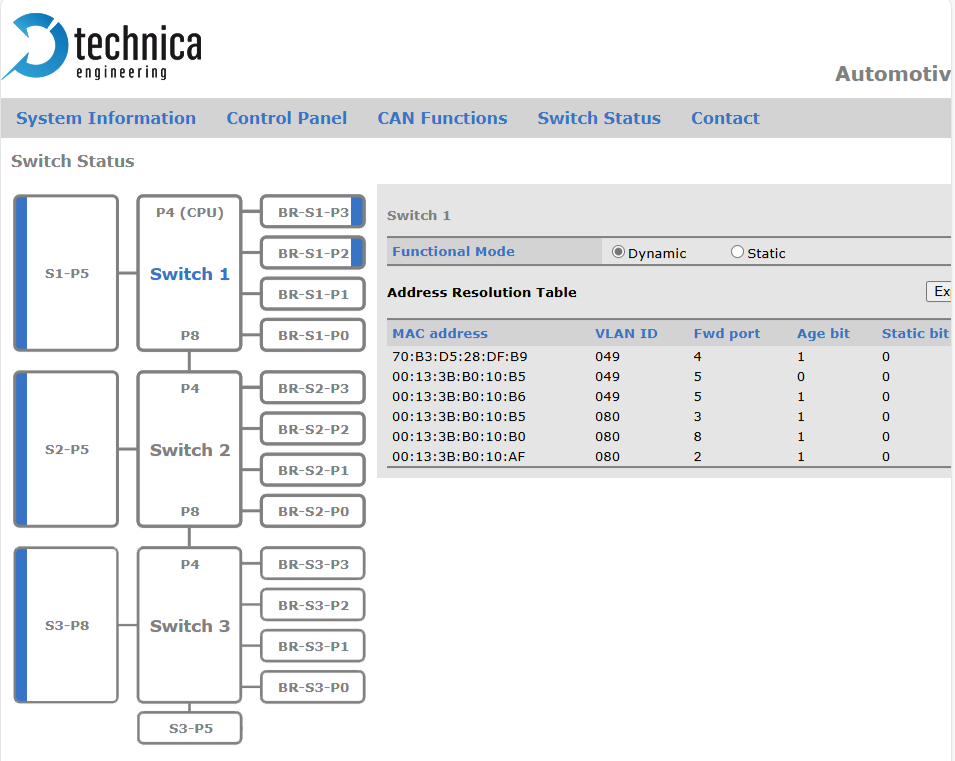
\includegraphics[width=0.8\textwidth]{figures/pictures/vlanconfig.PNG}
    \caption{VLAN Configuration.}
    \label{fig:mediagateway_setup3}
\end{figure}
\subsection{Task Report}
After realizing a simulated point to point connection in Part 1, this set of tasks revolved around advancing towards direct network communication through the Media Gateway with another physical workstation. The unconfigured media gateway will act as a layer 2 switch. Using the scripts from Part 1 as basis, they as well as the adapters had to be updated to reflect the new target.\\\\
The next task instructed the user to configure VLAN and build up a connection using it. Subsequently, a VLAN-based transmission path was configured, necessitating adjustments in the Media Gateway port settings (Figure 3). Upon correct VLAN implementation, packets containing payload data with increasing values were successfully transmitted and logged in Wireshark. The last task of this set, to access the webcam, was successful as well.\\\\
Significant challenges in this part included selecting the correct adapters and finding the correct port configuration, which was confusing at first, but after understanding the logic behind it, presented itself as a trivial matter. Another challenge was troubleshooting physical connectivity issues with an unresponsive webcam, which was later revealed to be the fault of a missing physical connection to the gateway.

\subsection{Conclusion}
In this package of Tasks the point to point connection to another workstation using the MediaGateway with the MAC address at first, then via VLAN-based transmission, was configured and established. The tasks helped further the understanding of VLAN and network traffic. There were some challenges in solving the tasks, but they were manageable to work around. 

%To Do: Screenshots einfügen; 





% A figure example:
%\begin{figure}[h]
    %\centering
    % \includegraphics[width=0.8\textwidth]{path/to/your/image.png}
    %\caption{Network diagram of the MediaGateway setup.}
    %\label{fig:mediagateway_setup}
%\end{figure}
